\documentclass{article}
\usepackage[a4paper, total={6in, 11in}]{geometry}
\usepackage{graphicx}
\usepackage{amsmath}
\usepackage{hyperref}

\title{DSC 180A Methodology Assignment 4}
\author{Issac Roy (\href{mailto:iroy@ucsd.edu}{iroy@ucsd.edu})}
\date{April 01 2005}

\begin{document}

\maketitle

\section{Deviations}
\subsection{Setup}

Consider a sample of $n$ values, $x_1, x_2, \ldots, x_n$, and let $\bar{x} = \frac{1}{n}\sum_{i=1}^n x_i$. Then, the sum of deviations from each $x_i$ to $\bar{x}$ is 0:

\begin{align*}
\sum_{i=1}^n (x_i - \bar{x}) &= \sum_{i=1}^n x_i - \sum_{i=1}^n \bar{x} \\
&= n\bar{x} - n\bar{x} \\
&= \boxed{0}
\end{align*}

\subsection{Runtime Analysis}

What is the asymptotic runtime of \texttt{standard\_deviation}, where $n$ is \texttt{len(xs)}?

\begin{verbatim}
def standard_deviation(xs):
    return (sum([(x - sum(xs) / len(xs)) ** 2 for x in xs]) / len(xs)) ** 0.5
\end{verbatim}

\begin{center}
\begin{tabular}{|c|c|}
\hline
$O(n)$ & $O(n^2)$ \\
\hline
$O(\log n)$ & $O(n \log n)$ \\
\hline
\end{tabular}
\end{center}

\section{Trivia}

How many of the following sentences (some of which are taken from \href{https://www.signupgenius.com/groups/true-or-false-questions.cfm}{here}) are true?

\begin{enumerate}
    \item Caesar Salad originates from Italy.
    \item Brazil is the only nation to have played in every World Cup finals tournament.
    \item The original Costco location is in San Diego.
\end{enumerate}

\section{Picture}

Here's a picture of my dog, ``Junior.''

\begin{center}
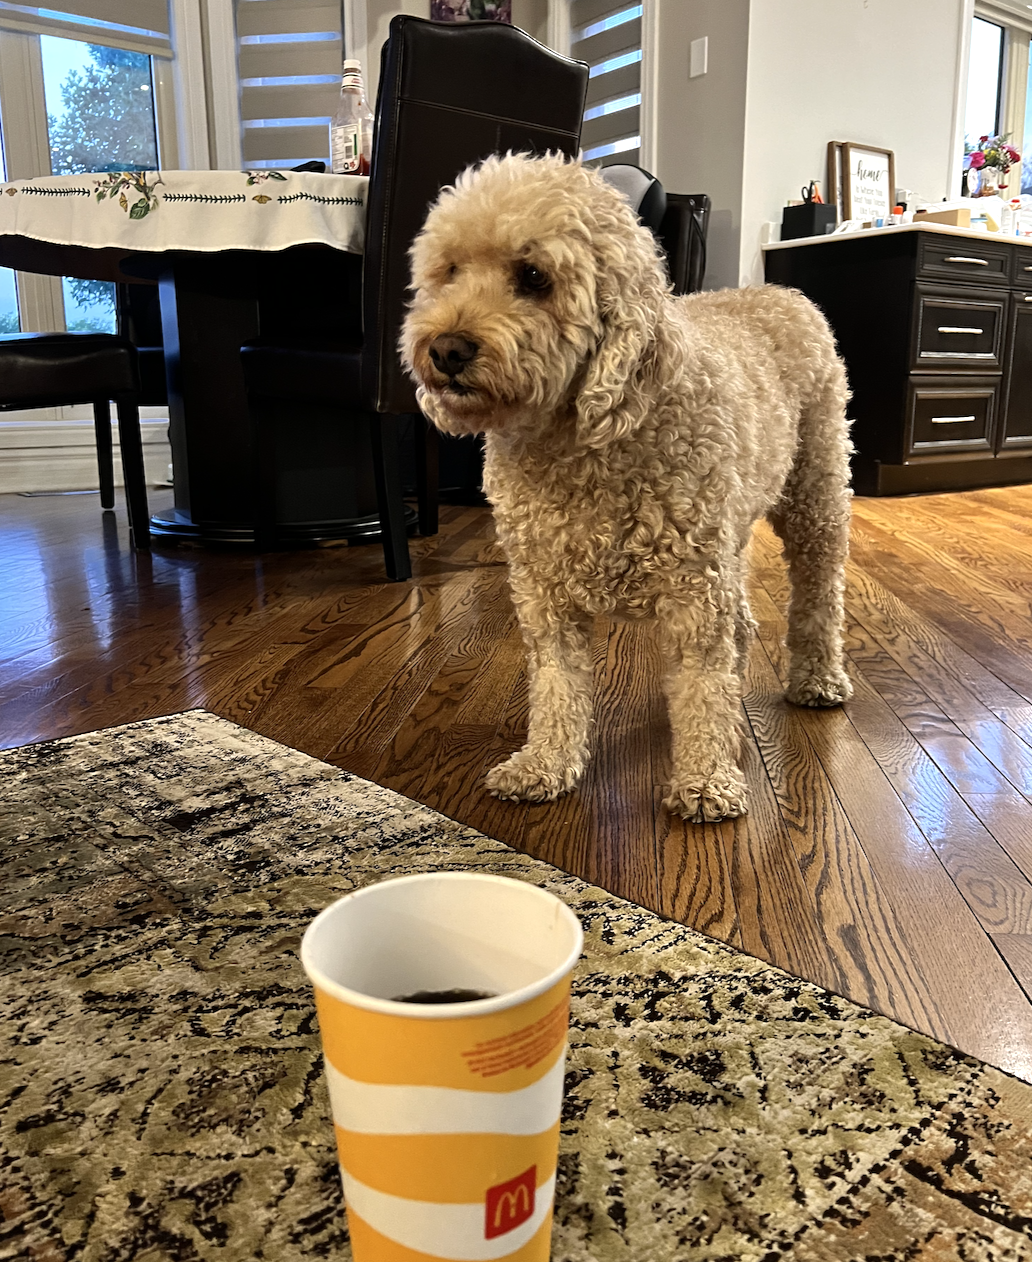
\includegraphics[width=0.3\textwidth]{junior.png}
\end{center}

\begin{itemize}
    \item He's 14 years old.
    \item He's a cockapoo.
\end{itemize}

\end{document}
